\documentclass{article}

\usepackage[utf8]{inputenc}
\usepackage{babel}
\usepackage{graphicx}
\usepackage{caption}
\usepackage{float}
\usepackage{color}
\usepackage{epigraph}
\usepackage[hang,flushmargin]{footmisc} 
\usepackage{tikz}
\usepackage{hyperref}
\hypersetup{pdfauthor={Cristian Adrián Ontivero}}
\usetikzlibrary{automata, positioning, arrows,
fit, % for the dashed boxes on Thompson's construction
calc
}
\tikzset{%
  node distance=3cm, % specifies the minimum distance between two nodes. Change if necessary.
  every state/.style={thick}, % sets the properties for each ’state’ node
  double distance=2.5pt,
  shorten >= 2pt, shorten <= 2pt,
  initial text=$ $,
  every edge/.style={%
    draw,->, >=stealth, auto, semithick
  }
}
\graphicspath{{imgs/}}

\definecolor{darkblue}{RGB}{49,130,189}

\newlength\tindent
\setlength{\tindent}{\parindent}
\setlength{\parindent}{0pt}
\renewcommand{\indent}{\hspace*{\tindent}}

%These tell TeX which packages to use.
\usepackage{array,epsfig}
\usepackage{amsmath}
\usepackage{amsfonts}
\usepackage{amssymb}
\usepackage{amsxtra}
\usepackage{amsthm}
\usepackage{mathrsfs}
\usepackage{color}

%Here I define some theorem styles and shortcut commands for symbols I use often
\theoremstyle{definition}
\newtheorem{defn}{Definition}
\newtheorem{thm}{Teorema}
\newtheorem{cor}{Corolario}
\newtheorem*{rmk}{Remark}
\newtheorem{lem}{Lema}
\newtheorem*{joke}{Joke}

\newtheorem{ex}{Example}
\newcommand{\exautorefname}{Ejemplo}

\newtheorem{exercise}{Ejercicio}
\newcommand{\exerciseautorefname}{Ejercicio}

\newtheorem{soln}{Solución}
\newtheorem{prop}{Proposición}

\newcommand{\lra}{\longrightarrow}
\newcommand{\ra}{\rightarrow}
\newcommand{\surj}{\twoheadrightarrow}
\newcommand{\graph}{\mathrm{graph}}
\newcommand{\bb}[1]{\mathbb{#1}}
\newcommand{\Z}{\bb{Z}}
\newcommand{\Q}{\bb{Q}}
\newcommand{\R}{\bb{R}}
\newcommand{\C}{\bb{C}}
\newcommand{\N}{\bb{N}}
\newcommand{\M}{\mathbf{M}}
\newcommand{\m}{\mathbf{m}}
\newcommand{\MM}{\mathscr{M}}
\newcommand{\HH}{\mathscr{H}}
\newcommand{\Om}{\Omega}
\newcommand{\Ho}{\in\HH(\Om)}
\newcommand{\bd}{\partial}
\newcommand{\del}{\partial}
\newcommand{\bardel}{\overline\partial}
\newcommand{\textdf}[1]{\textbf{\textsf{#1}}\index{#1}}
\newcommand{\img}{\mathrm{img}}
\newcommand{\ip}[2]{\left\langle{#1},{#2}\right\rangle}
\newcommand{\inter}[1]{\mathrm{int}{#1}}
\newcommand{\exter}[1]{\mathrm{ext}{#1}}
\newcommand{\cl}[1]{\mathrm{cl}{#1}}
\newcommand{\ds}{\displaystyle}
\newcommand{\vol}{\mathrm{vol}}
\newcommand{\cnt}{\mathrm{ct}}
\newcommand{\osc}{\mathrm{osc}}
\newcommand{\LL}{\mathbf{L}}
\newcommand{\UU}{\mathbf{U}}
\newcommand{\support}{\mathrm{support}}
\newcommand{\AND}{\;\wedge\;}
\newcommand{\OR}{\;\vee\;}
\newcommand{\Oset}{\varnothing}
\newcommand{\st}{\ni}
\newcommand{\wh}{\widehat}

\newcommand{\emptystr}{\varepsilon}
\newcommand{\emptylan}{\emptyset}
\newcommand{\pdv}[2]{\partial_{#1} \bigl(#2\bigr)}

%Pagination stuff.
\setlength{\topmargin}{-.3 in}
\setlength{\oddsidemargin}{0in}
\setlength{\evensidemargin}{0in}
\setlength{\textheight}{9.in}
\setlength{\textwidth}{6.5in}
\pagestyle{empty}

% Print today's date in ISO format (YYYY-MM-DD).
\def\isodate{\leavevmode\hbox{\the\year-\twodigits\month-\twodigits\day}}
\def\twodigits#1{\ifnum#1<10 0\fi\the#1}

\begin{document}
\begin{center}
  {\LARGE Down the Regular Expression Rabbit Hole}\\[.2cm]
  Cristian Adrián Ontivero \\[.05cm]%
  \isodate
\end{center}

\vspace{0.2 cm}
\section{Regular Expressions}
Regular expressions were introduced by Kleene, and may be inductively defined as follows:
\begin{defn}
Let $\Sigma$ be an alphabet. Then:
\begin{enumerate}
  \item $\emptyset, \emptystr$, and $a$, for $a \in \Sigma$ are regular expressions.
  \item If $R, S$ are regular expressions, then so are $R\cdot S, R+S$, and $R^*$.
\end{enumerate}
\end{defn}

%TODO

%Since regular languages are closed under intersection, union and
%complementation???, we can define \textit{extended} regular expressions. These
%are regular expressions which accept an additional inductive case, namely
%$f({\tt R}, {\tt S})$ is a regular expression, denoting any boolean function.

%which
%are no more ``powerful'' than simple regular expressions, but sometimes allow us
%to express a language more succinctly or intuitively.

%TODO

%Since ......, there is nothing that extended regular expressions can do but
%plain regular expressions cannot. Even so, they allow expressing certain
%languages in a more concise -- or intuitive -- way, and are interesting in their
%own right.

%Several algorithms have been designed to convert regular expressions into
%automata, and we will go through an overview in what follows.
%
%Algorithms based on the notion of position.
  %* Glushkov
  %* McNaughton \& Yamada
%Algorithms based on derivatives (or language left quotients)
  %* Derivatives.
    %- ``On-the-fly'' matching.
    %- Brzozowski's construction.
  %* Partial derivatives 
    %- Antimirov's construction.
  %* Cham. \& Ziadi

Brzozowski introduced the notion of derivatives of regular
expressions~\cite{Brz64}. Given a language $L$ over an alphabet $\Sigma$, and a
word $w \in \Sigma^*$, the derivative of $L$ with respect to $w$ is $D_w(L) = \{ t~|~wt\in L \}$. This is the same as the left
quotient set of $L$ with respect to $w$, sometimes denoted $w^{-1}(L)$.

\begin{defn}
(Brzozowski~\cite{Brz64}) Given a regular expression, and a symbol $a \in \Sigma$, the
derivative of the regular expression with respect to $a$ may be inductively
defined as follows:

\begin{minipage}{.4\textwidth}
\[
  \arraycolsep=2pt\def\arraystretch{1.4}
  \begin{array}{rl}
    D_{a}(\emptystr) &= \emptylan \\
    D_{a}(\emptylan) &= \emptylan \\
    D_{a}(b) &= \left\{ 
      \begin{array}{ll}
        \emptystr, &\text{if } b = a\\ 
        \emptylan, &\text{otherwise}
      \end{array}
    \right
\end{array}
\]
\end{minipage}%
\begin{minipage}{.4\textwidth}
\[
  \arraycolsep=2pt\def\arraystretch{1.4}
  \begin{array}{rl}
    D_{a}(R^*) &= (D_a R)R^* \\
    D_{a}(R+S) &= D_a R + D_a S \\
    D_{a}(RS) &= \left\{ 
      \begin{array}{ll}
        (D_a R)S + D_a S, &\text{if $R$ accepts $\emptystr$} \\ 
        (D_a R)S,         &\text{otherwise}
      \end{array}
        \right \\
\end{array}
\]
\end{minipage}%
\end{defn}

Although the set of derivatives of a regular expression may not be finite,
Brzozowski proved that its quotient modulo the ACI-axioms of the sum is, where
the ACI-axioms are:
\[
  \arraycolsep=2pt
  \begin{array}{rcl@{\hspace{4em}}l}
    r + (s + t) &=& (r + s) + t & \text{Associativity}\\
    r + s &=& s + r &\text{Commutativity}\\
    r + r &=& r &\text{Idempotence}
\end{array}
\]
\begin{defn}
Two regular expressions are said to be \textit{similar} if one can be converted
into the other by using only the ACI-axioms, and \textit{dissimilar} otherwise.
\end{defn}
Although that was Brzozowski's definition, some authors have exteded the list of
axioms used (e.g.\ see~\cite{ORT09}). 
The original equation for $D_a(RS)$ in \cite{Brz64} was slightly different, but
Antimirov~\cite{An96} noted that using that definition allows an infinite
sequence of regular expressions, even modulo the ACI-axioms. Using the
definition given circumvents the problem, and makes Brzozowski's finiteness
proof be correct without further changes.

\begin{ex}
Let $\tt E = {(a+b)}^*a{(a+b)}^2$ be a regular expression. For
simplicity let also $\tt R = a + b$. For every symbol of
the alphabet $\Sigma = \{{\tt a, b}\}$, take the derivative of {\tt E} with
respect to the symbol, and for each new regular expression found, do the same
until no new regular expression is found:

\begin{minipage}[t]{.5\textwidth}
\[
  \begin{array}{rcl}
    D_a(E) &=& D_a({(a+b)}^*)a{(a+b)}^2 + D_a(a{(a+b)}^2) \\
           &=& D_a{(a+b)}{(a+b)}^*a{(a+b)}^2 + {(a+b)}^2 \\
           &=& (\emptystr+\emptylan){(a+b)}^*a{(a+b)}^2 + {(a+b)}^2 \\
           &=& a{(a+b)}^2 + {(a+b)}^2 \\
           &=& E + R^2 \\
    D_b(E) &=& D_b({(a+b)}^*)a{(a+b)}^2 + D_b(a{(a+b)}^2) \\
           &=& E + \emptylan \\
           &=& E \\
\end{array}
\]
\end{minipage}%
\begin{minipage}[t]{.5\textwidth}
\[
  \begin{array}{rcl}
    D_a(E + R^2) &=& D_a(E) + D_a(R^2) \\
                 &=& E + R^2 + R \\
    D_b(E + R^2) &=& D_b(E) + D_b(R^2) \\
                 &=& E + R \\
    D_a(E + R^2 + R) &=& D_a(E) + D_a(R^2) + D_a(R)\\
                     &=& E + R^2 + R + \emptystr \\
    D_b(E + R^2 + R) &=& D_b(E) + D_b(R^2) + D_b(R)\\
                     &=& E + R + \emptystr\\
                     &\vdots&\\
                     & etc &\\
  \end{array}
\]
\end{minipage}

We use this to build a DFA recognizing $L({\tt E})$ where each regular
expression is a state. Deriving a regular expression {\tt r} with
respect to a symbol $c \in \Sigma$ gives a new regular expression, which
results from matching $c$ on the input string. In other words, $D_a(r) =
\delta(r, a)$. The state diagram of the DFA resulting from this process can be
seen in \autoref{fig:example-derivatives}.

\begin{figure}[ht] % ’ht’ tells LaTeX to place the figure ’here’ or at the top of the page
\centering % centers the figure
  \begin{tikzpicture}
    \tikzset{every state/.append style={rectangle, rounded corners}}
    \node[state, initial] (q0) {$E$};
    \node[state, right of=q0] (q1) {$E+R^2$};

    \node[state, above right=24pt and 48pt of q1] (q2) {$E + R^2 + R$};
    \node[state, below right=24pt and 60pt of q1] (q3) {$E+R$};

    \node[state, accepting, above right=0pt and 48pt of q2] (q4) {$E+R^2 + R + \emptystr$};
    \node[state, accepting, below right=0pt and 58pt of q2] (q5) {$E + R + \emptystr$};
    \node[state, accepting, above right=0pt and 66pt of q3] (q6) {$E + R^2 + \emptystr$};
    \node[state, accepting, below right=0pt and 76pt of q3] (q7) {$E+\emptystr$};

    \draw (q0) edge[loop above] node {b} (q0);
    \draw (q4) edge[loop above] node {a} (q4);
    \draw (q0) edge node {a} (q1);
    \draw (q1.0) edge node {a} (q2.180);
    \draw (q1.0) edge node[below] {b} (q3.180);

    \draw (q2) edge node {a} (q4.180);
    \draw (q2) edge node {b} (q5.180);

    \draw (q3) edge node {a} (q6.180);
    \draw (q3) edge[bend right=10] node {b} (q7);

    \draw (q4) edge node {b} (q5);
    \draw (q5) edge node {a} (q6);
    \draw (q5) edge[bend left=70] node {b} (q7);
    \draw (q6) edge[bend left=20] node {a} (q2);
    \draw (q6) edge[bend left=10] node {b} (q3);
    \draw (q7) edge[out=185, in=290] node {a} (q1);
    \draw (q7) edge[out=190, in=290] node {b} (q0);
    %\draw (c1) edge[bend left] node {1} (c0);
    %\draw (c1) edge[loop above] node {0} (c1);
  \end{tikzpicture}
  \caption{Brzozowski's derivative automaton for $E = {(a+b)}^*a{(a+b)}^2$.}\label{fig:example-derivatives}
\end{figure}
\end{ex}

Partial derivatives of regular expression are due to Antimirov~\cite{An96}. Just as
derivatives give a way to build a DFA, partial derivatives give a way to build
an NFA. Keeping with the example previously used, we take the partial
derivatives of $E$, and whatever other regular expression shows up in the
process:

\begin{minipage}{.5\textwidth}
\[
\arraycolsep=2pt\def\arraystretch{1.4}
  \begin{array}{rcl}
  \partial_a E &=& \pdv{a}{{(a+b)}^*}\cdot a{(a+b)}^2 \cup
    \pdv{a}{a{(a+b)}^2} \\
    &=& \bigl\{{(a+b)}^*a{(a+b)}^2, {(a+b)}^2\bigr\} \\
                                   &=& \bigl\{E, R^2\bigr\} \\
    \partial_a R^2 &=& \pdv{a}{a+b}\cdot {(a+b)} = \bigl\{R \bigr\} = \partial_b R^2 \\
  \end{array}
\]
\end{minipage}%
\begin{minipage}{.5\textwidth}
\[
\arraycolsep=2pt\def\arraystretch{1.4}
  \begin{array}{rcl}
    \partial_b E &=& \pdv{b}{{(a+b)}^*}\cdot a{(a+b)}^2 \cup \pdv{b}{a{(a+b)}^2} \\
                                  &=& \bigl\{E \bigr\} \\
    \\
    \partial_a R &=& \pdv{a}{a+b} = \bigl\{\emptystr \bigr\} = \partial_b R \\
  \end{array}
\]
\end{minipage}
\vspace{14pt}

The resulting NFA can be seen in \autoref{fig:example-pdv}.

\begin{figure}[ht] % ’ht’ tells LaTeX to place the figure ’here’ or at the top of the page
\centering % centers the figure
  \begin{tikzpicture}
    \tikzset{node distance=2.4cm}

    \node[state, initial] (q0) {$E$};
    \node[state, right of=q0] (q1) {$R^2$};
    \node[state, right of=q1] (q2) {$R$};
    \node[state, accepting, right of=q2] (q3) {$\emptystr$};

    \draw (q0) edge[loop above] node {a,b} (q0);
    \draw (q0) edge node {a} (q1);
    \draw (q1) edge node {a,b} (q2);
    \draw (q2) edge node {a,b} (q3);
  \end{tikzpicture}
  \caption{Antimirov's partial derivative automaton for $E = {(a+b)}^*a{(a+b)}^2$.}\label{fig:example-pdv}
\end{figure}

\section{Extended Regular Expressions}

\subsection{Final Remarks}
For a more recent treatment on Brzozowski's derivatives, see~\cite{ORT09}.

\newpage 
\bibliography{refs}
\bibliographystyle{unsrt}

\end{document}


